
\chapter{Como adicionar materiais}

\inputencoding{latin9}\lhead{Ap�ndice \thechapter: Como utilizar o software}\rhead{\thepage}

Para adicionar qualquer material ao simulador, � necess�rio clicar
em Arquivo->Import material, e escolher o arquivo desejado. � importante
lembrar que os arquivos devem ter o formato que ser� ensinado abaixo,
e a extens�o do arquivo deve ser '.constante', '.correlacao' ou '.interpolacao',
conforme o modelo escolhido.

\begin{figure}[H]
\begin{centering}
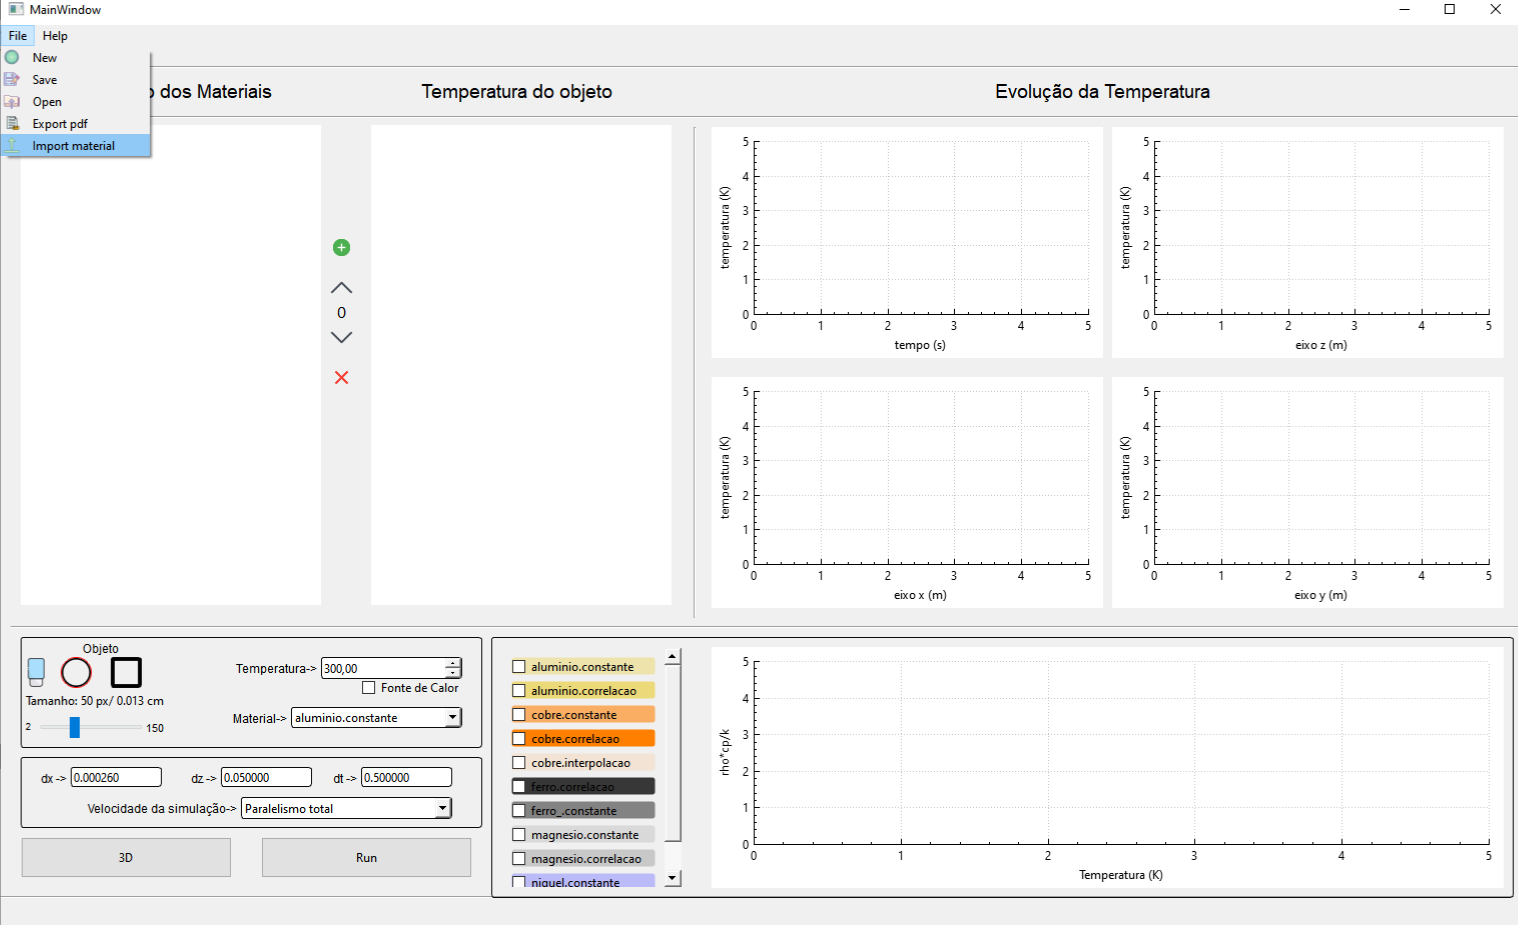
\includegraphics[scale=0.3]{../imagens/importar_material}
\par\end{centering}
\caption{Como adicionar um material no simulador. Primeiro seleciona Arquivo,
Import material. Uma janela ser� aberta, para o usu�rio escolher o
material.}

\end{figure}


\section{M�todo da correla��o ou constante}

Para adicionar um material que utilize m�todos de correla��o ou possu�
propriedades termof�sicas constantes, dever� ser criado um arquivo
com extens�o '.correlacao' ou '.constante', respectivamente.

O molde do arquivo � apresentado abaixo:

\noindent\fbox{\begin{minipage}[t]{1\columnwidth - 2\fboxsep - 2\fboxrule}%
\textcolor{gray}{RGBA:} 236 217 122 255

\textcolor{gray}{/// C1+C2{*}T }

\textcolor{gray}{Cp:} 2.753 0.000223

\textcolor{gray}{k:} 76.64 0.2633 0.0002

\textcolor{gray}{rho:} 0.7473 0.0002 0.0000005%
\end{minipage}}

Onde a primeira linha cont�m o RGBA do material, na linha do Cp, cada
valor � o valor das respectivas constantes, seguindo o modelo de correla��o
nas linhas comentadas ('///').M�todo da correla��o ou constante

\section{M�todo de interpola��o}

Para adicionar um material que utilize m�todos de interpola��o, dever�
ser criado um arquivo com extens�o '.interpolacao'.

O molde do arquivo � apresentado abaixo:

\noindent\fbox{\begin{minipage}[t]{1\columnwidth - 2\fboxsep - 2\fboxrule}%
\textcolor{gray}{RGBA:} 255 128 0 30 

\textcolor{gray}{rho:} 7.262 

\textcolor{gray}{Cp:} 7.925 

\textcolor{gray}{-T-{}-{}-k: }

100 0.2 

200 0.4 

300 0.5 

400 0.55 

500 0.6 

600 0.65 

700 0.7 

800 0.75 

900 0.8 %
\end{minipage}}

Onde a primeira linha cont�m o RGBA do material, nas linhas abaixo
cont�m rho e Cp. Abaixo da linha com T e k, s�o inseridos os valores
da temperatura, e a respectiva condutividade t�rmica (k). O usu�rio
pode adicionar quantas linhas desejar.
